This section describes the purpose, use, and intended user audience for the "Roam\_Bot". The Roam\_BOT is a unique system that allows users to implement pathfinding algorithms to test the efficiency of their software in real time using advanced technology. Educational users will be able to evaluate the effect of different algorithms to traverse and map the surrounding areas.

% This section provides a high-level statement of your product concept - what it is intended to do and how it is intended to be used. Include in this header paragraph, a brief synopsis of what is described here. For example, this header paragraph might say something like: "This section describes the purpose, use and intended user audience for the X product. X is a system that performs Y. Users of X will be able to Z..."

\subsection{Purpose and Use}
The Roam\_Bot should assist with learning to implement autonomous system software through real test simulations. Using an actual robotic system, software can be developed much more robustly to handle real-world obstacles. 

% This is where you describe in a brief, yet clear and concise, manner what your product should do and how you expect it should be used.

\subsection{Intended Audience}
The majority of the Roam\_Bot user base will be students. It will be made publicly available to the public for multiple learning institutions across the University of Texas at Arlington. Our system will be intended for the general purpose testing of navigation software.

% This is where you describe the intended audience(s) of your product. If this product were to be made available publicly or commercially, who would purchase or use it? Is the product designed for a particular customer, or an overall class of customers? Is it intended for general use, or is it a specific component of a more complex system?

%%%%%%%%%%%%%%%%%%%%%%%%%%%%%%%%%%%%%%%%%%%%%%%%%%%%%%%%%%%%%%%%%%%%%%%%%%%%
%   Change the graphic here. Put your image in the 'images' folder
%   and update the name from 'images/test_image' to your image name
% \begin{figure}[h!]
% 	\centering
%    	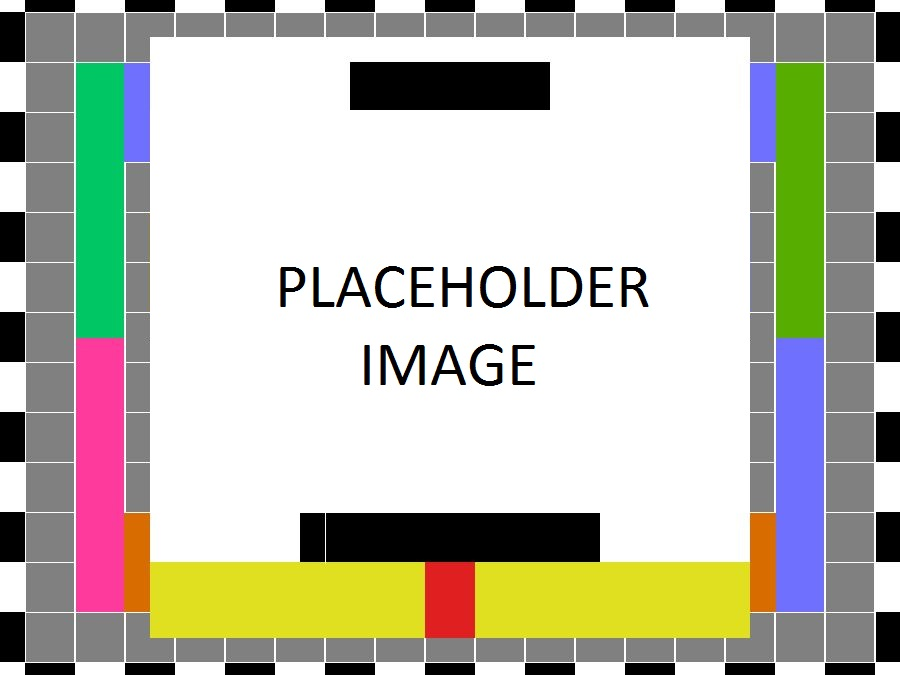
\includegraphics[width=0.60\textwidth]{images/test_image}
%     \caption{X conceptual drawing} % Be sure to change the caption!
% \end{figure}
